\documentclass[conference]{IEEEtran}
\usepackage{graphicx}
\usepackage{amsmath}
\usepackage{amssymb}
\usepackage{booktabs}
\usepackage{cite}
\usepackage{url}
\graphicspath{{../figures/}}

\begin{document}

\title{Flight Delay Prediction with Entity Embeddings and a Multilayer Perceptron:\\Phase 2 --- Deep Learning}

\author{
\IEEEauthorblockN{Asad Ali, Divyansh Bhartia, Vikrant Yadav, Mayank Pillai, Prashant Raj}
\IEEEauthorblockA{CSAI Project 21\\
Deep Learning}
}

\maketitle

\begin{abstract}
We extend our Phase 1 flight delay study with a deep learning model. The task is unchanged: predict, before
departure, whether a flight from a New York City airport in 2013 will arrive 15 or more minutes late. We train a
compact multilayer perceptron (MLP) with learned entity embeddings for the carrier, origin and destination, on the
same leakage-free features and date-based split as Phase 1. The network has 15{,}361 parameters and is
regularised with dropout, decoupled weight decay and early stopping. On the November--December test set it reaches
a PR AUC of 0.386 (random baseline 0.258) and ROC AUC of 0.653, between Logistic Regression (0.376) and XGBoost
(0.391), and is stable across five random seeds ($0.385 \pm 0.003$). Its raw probabilities are the best
calibrated of all models (Brier score 0.182, against 0.188 for calibrated XGBoost). An ablation study over five
seeds shows that the recent delay-history features matter most (PR AUC falls from 0.3845 to 0.3575 without them), while
embeddings perform on par with one-hot encoding. Finally, an offline what-if analysis finds a lower-risk departure
slot for 92.7\% of the highest-risk flights, mostly two hours earlier.
\end{abstract}

\begin{IEEEkeywords}
flight delay prediction, deep learning, entity embeddings, multilayer perceptron, dropout, calibration, ablation
\end{IEEEkeywords}

\section{Introduction}
Flight delays cost airlines and passengers time and money and spread through the network as late aircraft make
later flights late. In Phase 1 we built a leakage-free pipeline that predicts, before departure, whether a flight
will arrive at least 15 minutes late, and compared Logistic Regression with XGBoost. XGBoost was best, with a test
PR AUC of 0.391.

Phase 2 asks whether a deep learning model can learn the same patterns, and what its parts contribute. The
Project~21 brief suggests a compact MLP with learned embeddings for airline, origin and destination; a temporal
model is optional and was not used. Our contributions are:
\begin{itemize}
\item an MLP with entity embeddings trained on exactly the Phase 1 features, split and metrics, so that the
comparison with the Phase 1 models is fair;
\item a regularisation setup (dropout, AdamW weight decay, early stopping) and a stability check over five seeds;
\item an ablation study of the embeddings, categorical inputs, history features and regularisation;
\item a calibration analysis, a look at what the embeddings learned, and an offline what-if rescheduling analysis
with explicit assumptions.
\end{itemize}

\section{Deep Learning Literature Review}
\textbf{Deep learning for flight delays.} Sternberg \emph{et al.}~\cite{sternberg2017review} review flight delay
prediction and note a shift from statistical models towards machine learning. Kim \emph{et al.}~\cite{kim2016deep}
apply recurrent neural networks to day-to-day airport delay sequences, showing that deep models can capture delay
dynamics when ordered history is available.

\textbf{Multilayer perceptrons.} An MLP stacks linear layers and non-linear activations and is trained by
back-propagation of the loss gradient~\cite{rumelhart1986learning}. Rectified linear units
(ReLU)~\cite{nair2010rectified} avoid saturating gradients and are the default hidden activation.

\textbf{Entity embeddings.} Learned dense vectors for discrete symbols were popularised for words by Mikolov
\emph{et al.}~\cite{mikolov2013distributed}. Guo and Berkhahn~\cite{guo2016entity} apply the same idea to
categorical variables in tabular data: each category is mapped to a trainable vector, so that categories with
similar effects can end up close together and share statistical strength. This is the basis of our carrier,
origin and destination inputs.

\textbf{Regularisation and optimisation.} Dropout~\cite{srivastava2014dropout} randomly removes hidden units during
training to reduce co-adaptation and overfitting. Adam~\cite{kingma2015adam} adapts the step size per parameter;
AdamW~\cite{loshchilov2019decoupled} decouples weight decay from the gradient update, which makes L2-style
regularisation behave as intended. Early stopping~\cite{prechelt1998early} keeps the model from the epoch with the
best validation score.

\textbf{Deep learning versus trees on tabular data.} Several studies find that gradient-boosted trees such as
XGBoost~\cite{chen2016xgboost} still match or beat deep networks on medium-sized tabular data
\cite{grinsztajn2022tree,shwartz2022tabular}. Reasons include irregular target functions, uninformative features
and the rotation invariance of MLPs. We therefore treat XGBoost as a strong reference, not a weak baseline.

\textbf{Calibration.} Guo \emph{et al.}~\cite{guo2017calibration} show that modern neural networks are often
over-confident and propose temperature scaling, which divides the logits by one learned constant. Isotonic
regression~\cite{zadrozny2002transforming} is the non-parametric alternative we used in Phase 1.

\section{Dataset and Preprocessing}
\subsection{Data, features and split}
We use the Flights 2013 dataset (\texttt{nycflights13}~\cite{nycflights13}) with the Phase 1 pipeline unchanged:
327{,}346 completed flights, 24.5\% delayed; all post-departure fields removed; features for calendar and schedule
(weekend flag, distance, and cyclic $\sin/\cos$ encodings of the departure hour, arrival hour and day of week),
airport congestion (flights scheduled from the origin in the same hour and on the same day, counted on the full
schedule including later-cancelled flights) and recent history (the share of delayed flights over the previous
seven days for the carrier, origin, destination and route, today excluded). The data are split by date: train
January--August (217{,}727 flights, 26.4\% delayed), validation September--October (55{,}628, 15.7\%) and test
November--December (53{,}991, 25.8\%).

\subsection{Preprocessing for the network}
\textbf{Categorical inputs.} Carrier, origin and destination are mapped to integer ids built from the training set
only. Id~0 is reserved for categories never seen in training; 57 test flights go to such a destination and use
this shared ``unknown'' vector.

\textbf{Numeric inputs.} The 14 numeric features are standardised to zero mean and unit variance with training
statistics; missing history values (days without history) are filled with the training mean first.

\textbf{Class imbalance.} Unlike Phase 1, the network is trained with the plain binary cross-entropy, without class
weights. Weighting changes the predicted probabilities but not their ranking, so PR and ROC AUC are barely affected,
while unweighted training keeps the probabilities close to the true delay rate.

\section{Architecture}
For a flight with numeric vector $x \in \mathbb{R}^{14}$ and category ids $c_1, c_2, c_3$, each id selects a row of an
embedding matrix $E_j$, giving vectors of size 8 (carrier, 17 ids), 2 (origin, 4 ids) and 16 (destination, 103
ids). The sizes are small and grow with the number of categories. The input is the concatenation
\begin{equation}
h_0 = [\,x;\; E_1[c_1];\; E_2[c_2];\; E_3[c_3]\,] \in \mathbb{R}^{40}.
\end{equation}
Two hidden layers with ReLU and dropout ($p=0.3$) follow,
\begin{equation}
h_k = \mathrm{Dropout}\big(\mathrm{ReLU}(W_k h_{k-1} + b_k)\big), \quad k = 1, 2,
\end{equation}
with 128 and 64 units, and a linear output gives the logit $z = w^\top h_2 + b$ and the probability
$\hat p = \sigma(z)$. The model has 15{,}361 parameters, of which 1{,}792 are embedding weights. It is trained to
minimise the binary cross-entropy
\begin{equation}
\mathcal{L} = -\frac{1}{N}\sum_{i} \big[y_i \log \hat p_i + (1-y_i)\log(1-\hat p_i)\big].
\end{equation}
The embeddings are learned jointly with the rest of the network by back-propagation, so they encode whatever
differences between categories help the prediction.

\section{Training and Regularisation}
We use AdamW~\cite{loshchilov2019decoupled} with learning rate $10^{-3}$ and weight decay $10^{-4}$, mini-batches of
1{,}024 flights, and at most 30 epochs. After each epoch we compute the validation PR AUC and keep the best
weights; training stops after five epochs without improvement~\cite{prechelt1998early}. Models are implemented in
PyTorch~\cite{paszke2019pytorch} and trained on a laptop CPU in a few seconds per model.

Fig.~\ref{fig:learning} shows a typical run. The training loss keeps falling, but the validation PR AUC peaks at
epoch 4 and then declines: after a few epochs the network starts to fit patterns specific to the training months.
Early stopping, dropout and weight decay limit this overfitting.

\begin{figure}[t]
\centering
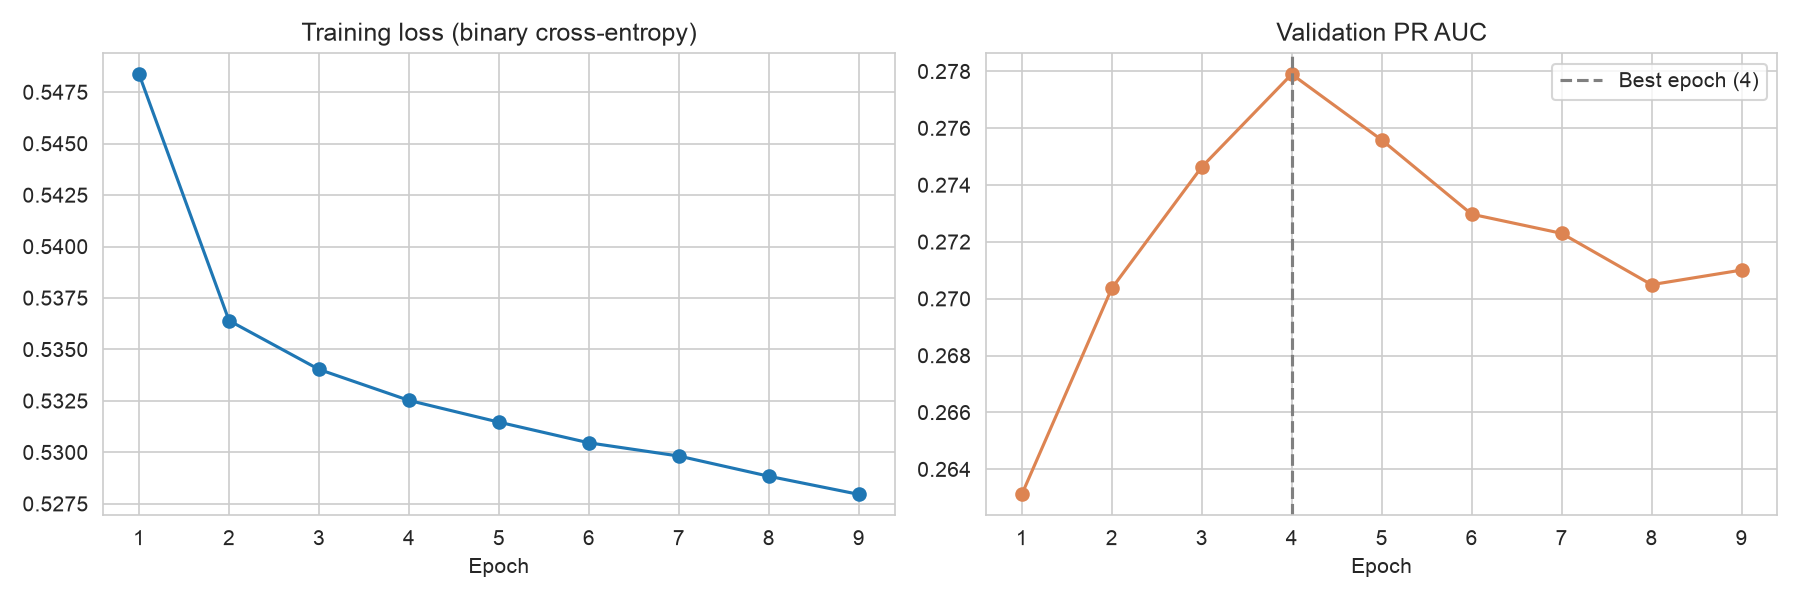
\includegraphics[width=\columnwidth]{learning_curves.png}
\caption{Training loss and validation PR AUC per epoch (seed 0). The best epoch (4) is kept.}
\label{fig:learning}
\end{figure}

\section{Technical Validation}
\subsection{Stability across seeds}
Weight initialisation, batch order and dropout are random. Over five seeds the test PR AUC is
$0.3845 \pm 0.0027$ (range 0.380--0.387) and the ROC AUC 0.649--0.653, so differences smaller than about 0.005
between configurations should not be read as real.

\subsection{Comparison with Phase 1}
Table~\ref{tab:results} and Fig.~\ref{fig:curves} compare the MLP (seed 0) with the Phase 1 models on the test set.
The MLP clearly beats Logistic Regression and is slightly behind XGBoost in PR AUC, ROC AUC and recall at 50\%
precision (9.4\% vs 11.1\% of delayed flights). This matches the literature on tabular data
\cite{grinsztajn2022tree,shwartz2022tabular}: with 14 engineered features and three categorical inputs, boosted
trees remain very strong.

\begin{table}[t]
\centering
\caption{Test set results (November--December 2013)}
\label{tab:results}
\setlength{\tabcolsep}{4pt}
\begin{tabular}{lcccc}
\toprule
Model & PR AUC & ROC AUC & Rec@P0.5 & Brier \\
\midrule
Random guess & 0.258 & 0.500 & -- & -- \\
Log. Regression & 0.376 & 0.645 & 0.059 & 0.228 \\
XGBoost & \textbf{0.391} & \textbf{0.656} & \textbf{0.111} & 0.219 \\
MLP (embeddings) & 0.386 & 0.653 & 0.094 & \textbf{0.182} \\
\bottomrule
\end{tabular}
\end{table}

\begin{figure}[t]
\centering
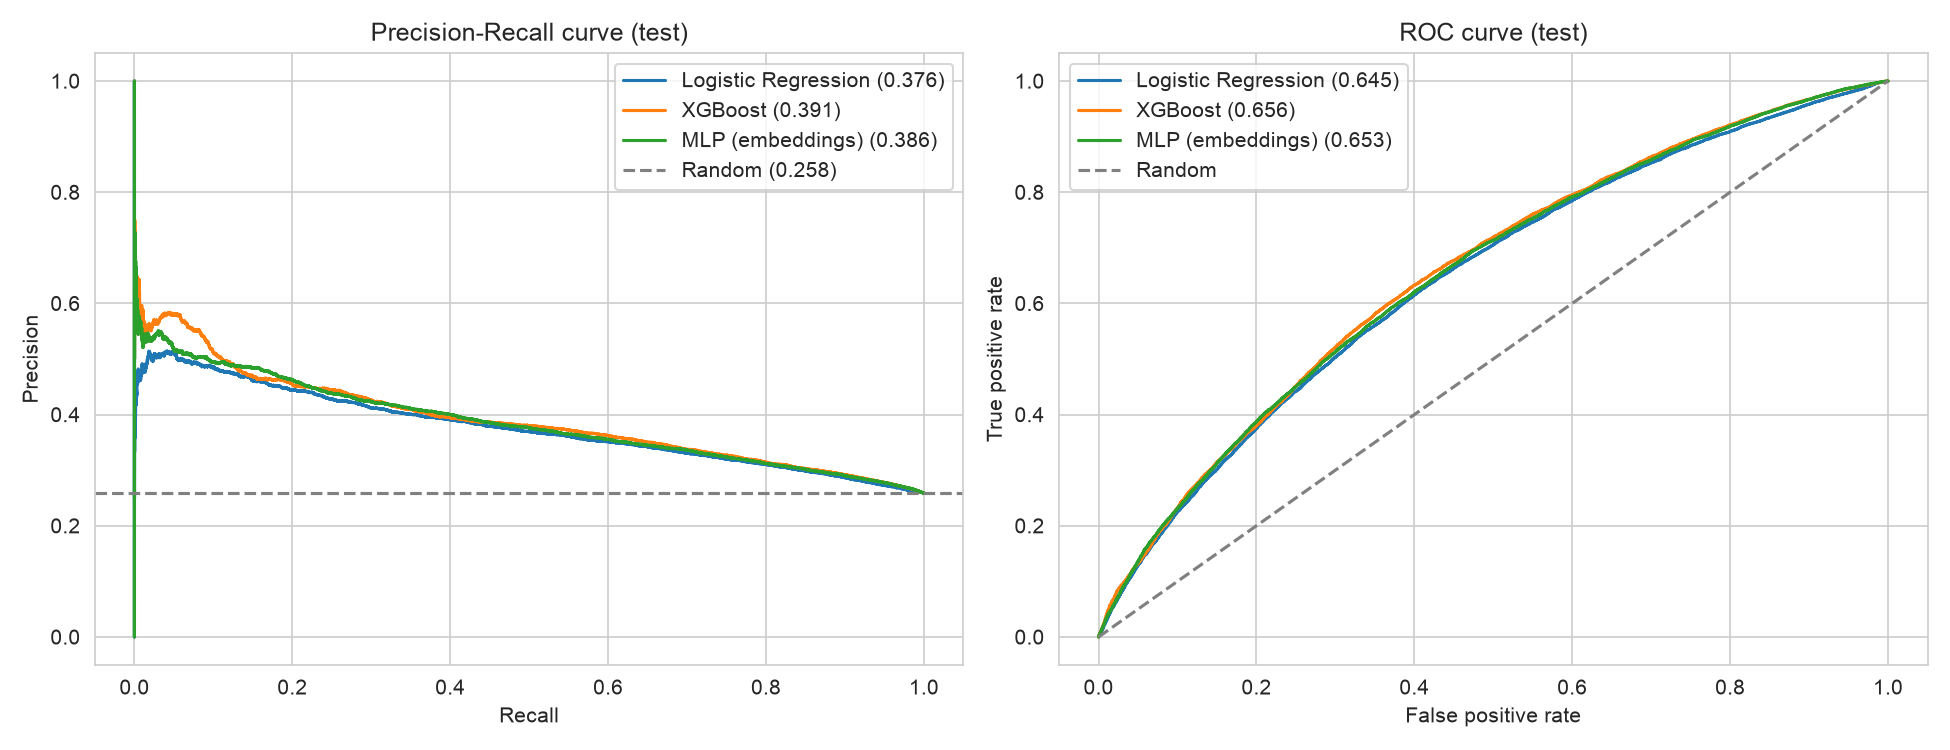
\includegraphics[width=\columnwidth]{pr_roc_curves.png}
\caption{Precision--recall and ROC curves on the test set.}
\label{fig:curves}
\end{figure}

\subsection{Calibration}
Without class weights, the MLP's raw probabilities are already well calibrated (Fig.~\ref{fig:calib}): its Brier
score of 0.182 is the best of all models, and its mean prediction (0.244) is close to the test delay rate
(0.258). We also fitted temperature scaling~\cite{guo2017calibration} on the validation set. The learned
temperature $T = 0.785$ \emph{sharpened} the probabilities and lowered their mean to 0.203, raising the Brier score
to 0.185. The cause is the seasonal shift: September--October had far fewer delays (15.7\%) than
November--December (25.8\%), so any calibration fitted on them pulls predictions down. The isotonic-calibrated
XGBoost from Phase 1 suffers from the same effect (Brier 0.188, mean prediction 0.175). We therefore keep the
MLP's raw probabilities.

\begin{figure}[t]
\centering
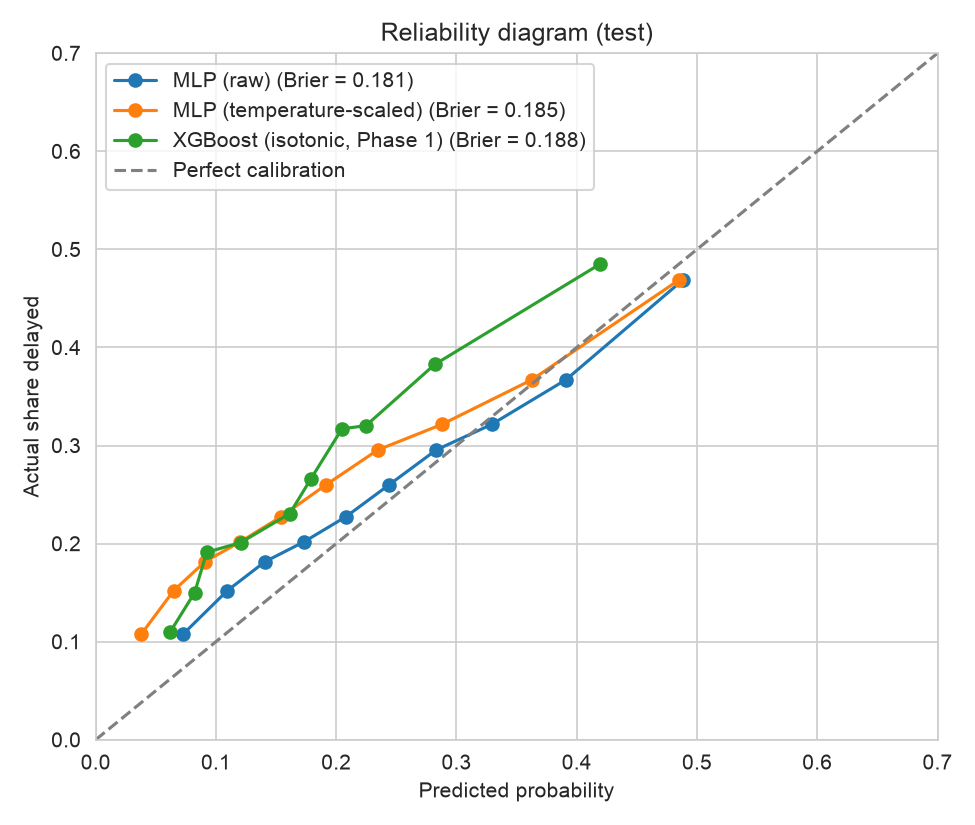
\includegraphics[width=0.85\columnwidth]{calibration.png}
\caption{Reliability diagram on the test set.}
\label{fig:calib}
\end{figure}

\section{Ablation Study}
Each variant was trained with five seeds; Table~\ref{tab:ablation} and Fig.~\ref{fig:ablation} report the mean test
PR AUC with its standard deviation.

\begin{table}[t]
\centering
\caption{Ablation study (5 seeds, test set)}
\label{tab:ablation}
\setlength{\tabcolsep}{4pt}
\resizebox{\columnwidth}{!}{%
\begin{tabular}{lccc}
\toprule
Variant & Val PR AUC & Test PR AUC & Test ROC \\
\midrule
Full model (emb.) & \textbf{0.2730} & 0.3845 $\pm$ 0.0027 & 0.6517 \\
One-hot, no emb. & 0.2691 & 0.3862 $\pm$ 0.0037 & 0.6565 \\
No categorical & 0.2725 & 0.3857 $\pm$ 0.0041 & 0.6553 \\
No history & 0.2679 & 0.3575 $\pm$ 0.0017 & 0.6248 \\
No dropout / w.\ decay & 0.2687 & 0.3826 $\pm$ 0.0061 & 0.6499 \\
\bottomrule
\end{tabular}}
\end{table}

\begin{figure}[t]
\centering
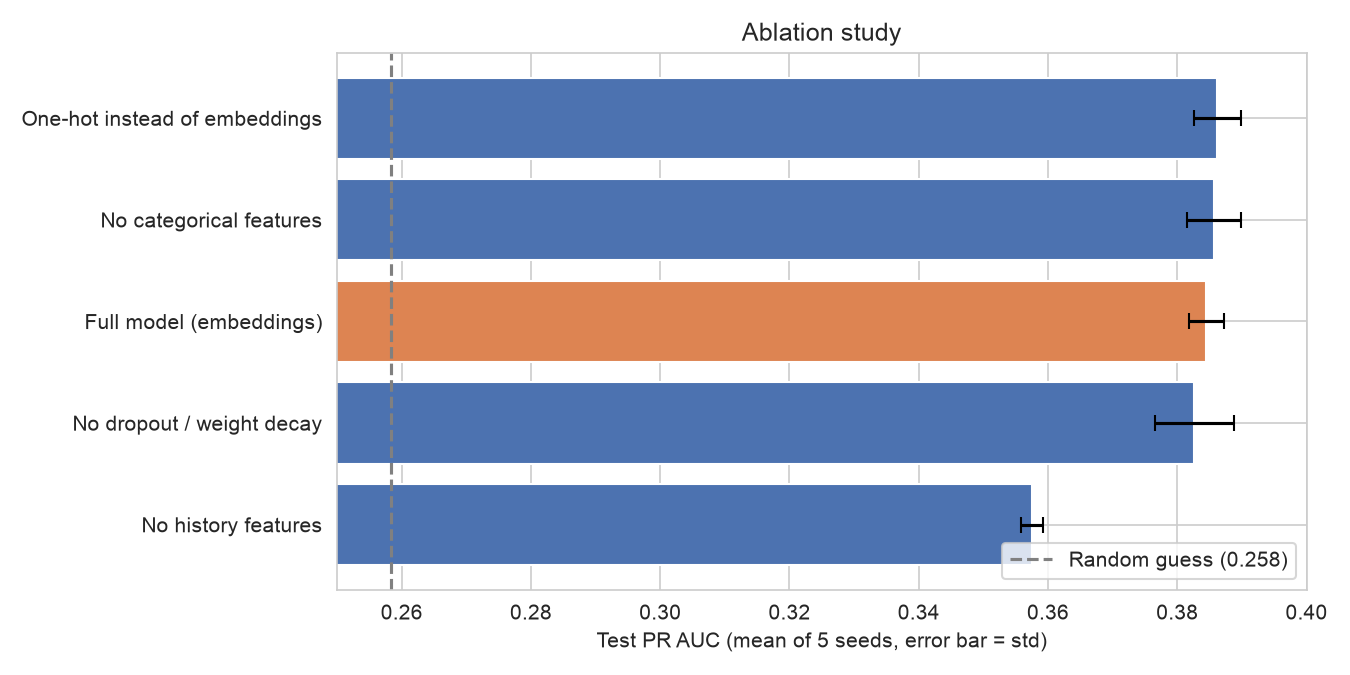
\includegraphics[width=\columnwidth]{ablation.png}
\caption{Ablation study: mean test PR AUC over five seeds (error bars: one standard deviation).}
\label{fig:ablation}
\end{figure}

\begin{itemize}
\item \textbf{History features} are by far the most important input: removing them lowers the test PR AUC from
0.3845 to 0.3575 and the ROC AUC from 0.6517 to 0.6248.
\item \textbf{Embeddings} perform on par with one-hot encoding and with no categorical inputs at all; all three are
within one standard deviation. The recent delay rates of the carrier, origin, destination and route already
summarise most of what the categories add.
\item \textbf{Regularisation} gives a small gain and, more clearly, more stable results: without dropout and weight
decay the seed-to-seed standard deviation roughly doubles (0.0061 vs 0.0027).
\end{itemize}
The full model has the best validation PR AUC, which is how it was chosen; the test differences between the first
three variants are within noise.

\section{What Did the Embeddings Learn?}
Fig.~\ref{fig:embed} projects the eight-dimensional carrier embeddings onto their first two principal components.
The first component correlates only weakly with each carrier's training delay rate ($r = -0.25$). This agrees with
the ablation: because the carrier's recent delay rate is already an input, the embeddings do not need to encode a
carrier's overall delay level and instead capture smaller differences, for example in how a carrier's delays
depend on the time of day. Carrier OO, with only seven training flights, is an outlier with an unreliable delay
rate.

\begin{figure}[t]
\centering
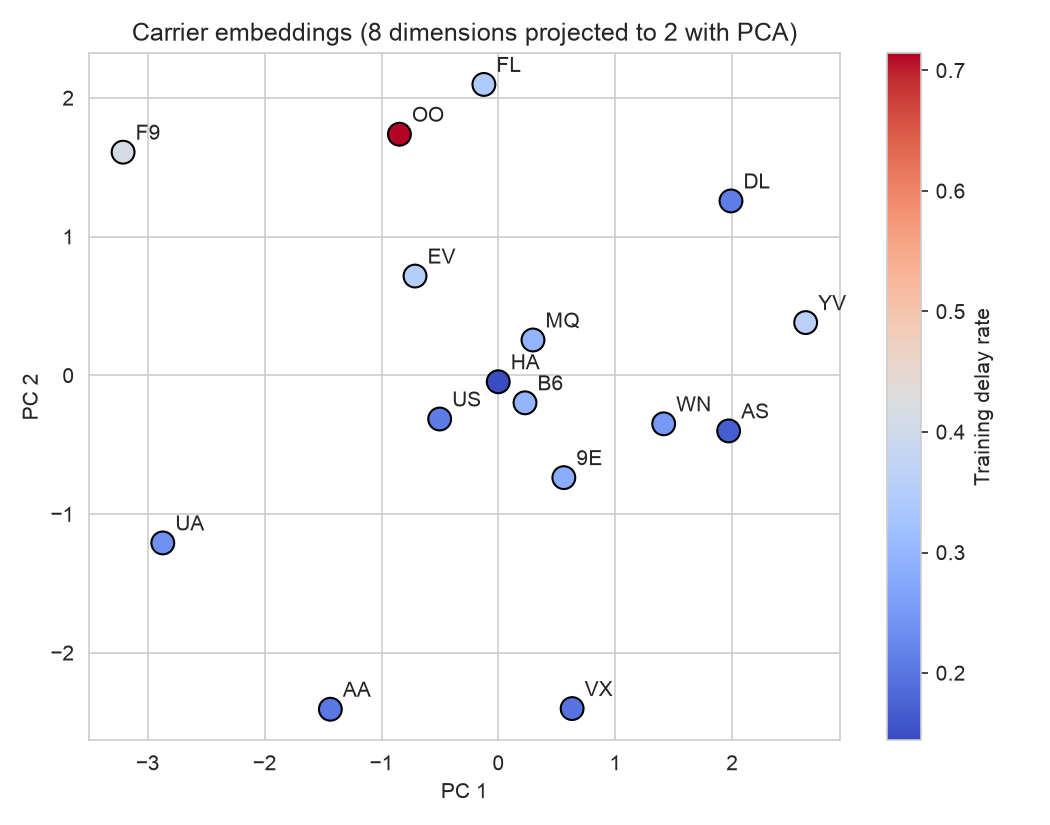
\includegraphics[width=0.85\columnwidth]{carrier_embeddings.png}
\caption{Carrier embeddings projected to two dimensions with PCA, coloured by training delay rate.}
\label{fig:embed}
\end{figure}

\section{What-If Rescheduling Analysis}
The Project 21 brief asks for an offline rescheduling analysis based on explicit assumptions. We take the 10\% of
test flights with the highest predicted risk (5{,}400 flights, risk $\ge 0.429$) and re-score each one with its
departure moved by $-2$, $-1$, $+1$ or $+2$ hours, assuming that: the flight stays on the same day, departs between
05:00 and 23:59 and does not arrive after midnight; the arrival moves by the same amount; route, carrier, date and
history features are unchanged; congestion is recomputed for the new hour; flights are moved one at a time; and
crews, aircraft rotations, gates and passengers are ignored. A move is recommended only if it lowers the predicted
risk.

Under these assumptions, 92.7\% of high-risk flights have a lower-risk slot, and for 40.7\% the risk falls by at
least five percentage points. The mean predicted risk of the group falls from 0.488 to 0.441. The most common
recommendation is to depart two hours earlier (3{,}651 flights), which reflects the build-up of delays during the
day (Fig.~\ref{fig:whatif}). These are model-based estimates of association, not causal effects: moving thousands of
flights would itself change congestion and delays.

\begin{figure}[t]
\centering
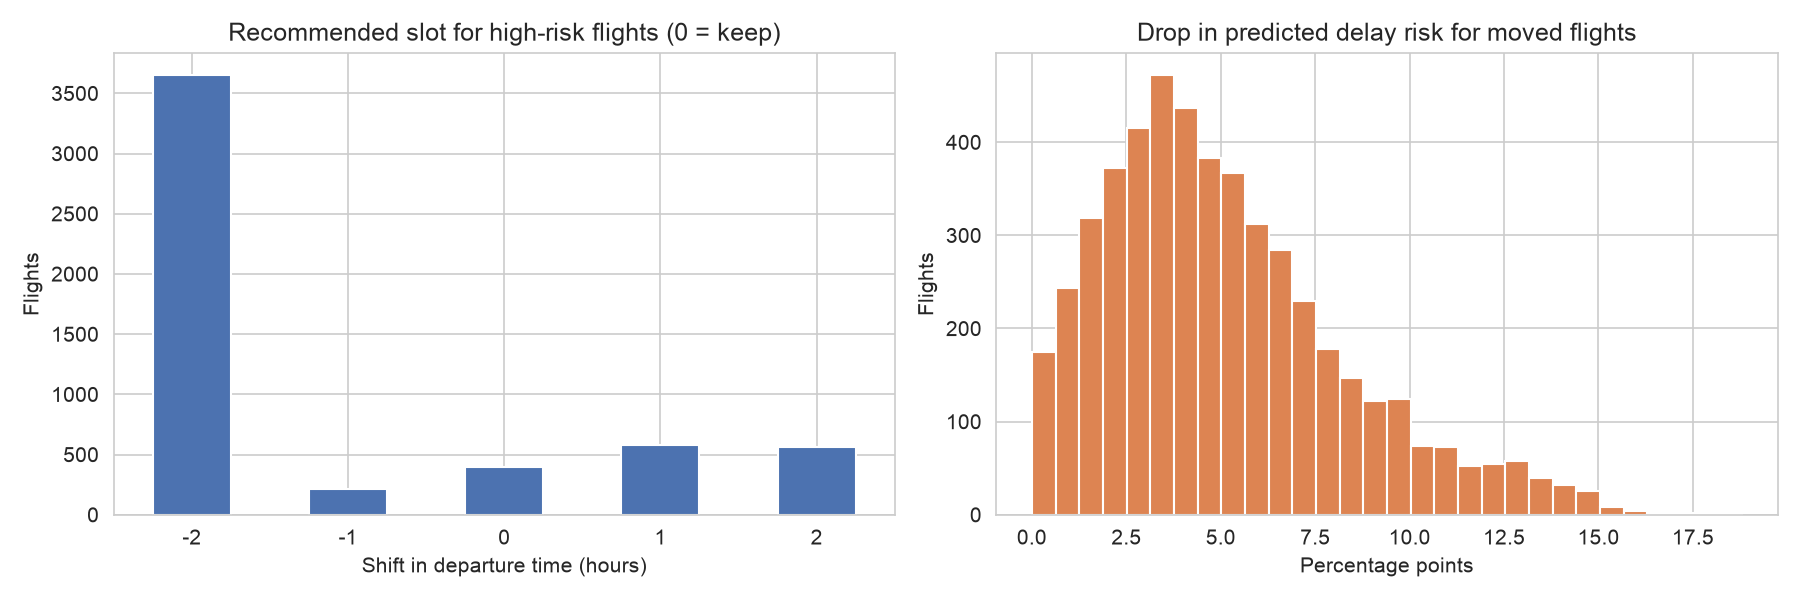
\includegraphics[width=\columnwidth]{what_if.png}
\caption{What-if analysis: recommended shift for high-risk flights (left) and the drop in predicted risk for moved
flights (right).}
\label{fig:whatif}
\end{figure}

\section{Discussion and Limitations}
The MLP learns the same signal as the Phase 1 models and gives the best-calibrated probabilities, but it does not
beat XGBoost in ranking quality. Most of the predictive power comes from the engineered history features, not from
the embeddings. Pre-departure prediction is limited by causes the data do not contain, such as weather, air traffic
control and late inbound aircraft. Other limitations are the single year and city, the seasonal difference between
validation and test months, and the simple, non-causal what-if analysis. We did not build a hybrid ML--DL model,
and the optional temporal model was left out.

\section{Conclusion and Future Work}
A compact MLP with entity embeddings, trained on leakage-free features with a date-based split, reaches a test PR
AUC of 0.386, close to XGBoost (0.391), with the best-calibrated probabilities of all models and stable results
across seeds. The ablation study shows that recent delay history drives the predictions and that embeddings add
little beyond it. Natural next steps are forecast weather inputs, a sequence model over the ordered history of each
aircraft or airport, and a hybrid that feeds learned embeddings to a tree model.

\bibliographystyle{IEEEtran}
\bibliography{references}

\end{document}
